\vspace{0.5em}
\section{Methodology: DP-ES}
\label{sec:methodology}
\enlargethispage{2\baselineskip}

\noindent\textbf{Problem Formulation.}
Let $\calD = \{(x_i, y_i)\}_{i=1}^n$ be a private dataset where $x_i$ represents task inputs and $y_i$ represents desired outputs (e.g., question-answer pairs). Let $\calP$ denote the space of natural language prompts. Our goal is to find a prompt $p^* \in \calP$ that maximizes task performance:
\begin{equation}
p^* = \arg\max_{p \in \calP} f(p, \calD)
\end{equation}
where $f: \calP \times \calD \to \R$ measures prompt quality (e.g., accuracy on $\calD$).

\noindent\textbf{Privacy requirement:} The optimization algorithm must satisfy $(\eps, \delta)$-differential privacy with respect to $\calD$, ensuring that any single record $(x_i, y_i)$ has bounded influence on the output prompt.

\begin{table}[t]
\centering
\scriptsize
\setlength{\tabcolsep}{3pt}
\begin{tabular}{cl@{\qquad}cl}
\toprule
$\calD,n$ & private data, size & $K,T$ & population, rounds \\
$b,q$ & batch size, $q=b/n$ & $z$ & Gaussian noise multiplier \\
$\widetilde{s}_p$ & privatized score & $\beta$ & Gumbel smoothing scale \\
\bottomrule
\end{tabular}
\caption{Notation used in DP-ES.}
\label{tab:notation}
\end{table}

\vspace{-0.5em}
\begin{definition}[$(\eps, \delta)$-Differential Privacy]
\label{def:dp}
A randomized algorithm $\calM: \calD \to \calO$ satisfies $(\eps, \delta)$-DP if for all neighboring datasets $\calD \sim \calD'$ (differing in one record) and all measurable sets $S \subseteq \text{Range}(\calM)$:
\vspace{-0.8em}
\begin{equation}
\Prob[\calM(\calD) \in S] \leq e^\eps \cdot \Prob[\calM(\calD') \in S] + \delta
\end{equation}
\end{definition}

\vspace{-0.5em}
\noindent\textbf{DP-ES Algorithm Overview.}
DP-ES (Algorithm~\ref{alg:dpes}) employs an evolution strategy with three key components:

\begin{enumerate}
    \vspace{-0.8em}
    \item \textbf{Mutation:} Generate prompt variations using an LLM (privacy-free)
    \vspace{-0.8em}
    \item \textbf{DP Evaluation:} Score prompts on $\calD$ with calibrated noise
     \vspace{-0.8em}
    \item \textbf{Selection:} Select top prompts from privatized scores (Gumbel-smoothed or deterministic)
\end{enumerate}

\begin{nolinenumbers}
\begin{algorithm}[t]
\caption{DP-ES: Differentially Private Evolution Strategies}
\label{alg:dpes}
\small
\begin{algorithmic}[1]
\REQUIRE Private dataset $\calD$, privacy budget $(\eps_{\text{total}}, \delta)$, initial prompt $p_0$, population size $K$, iterations $T$
\ENSURE Optimized prompt $p^*$ with $(\eps_{\text{total}}, \delta)$-DP
\STATE Initialize population $\mathcal{P}_0 \leftarrow \{p_0\}$
    \STATE Calibrate $z$ for $T K$ sampled-Gaussian scores \COMMENT{RDP accountant}
\FOR{$t = 1$ to $T$}
    \STATE \textcolor{blue}{// Phase 1: Privacy-free mutation}
    \FOR{each $p \in \mathcal{P}_{t-1}$}
        \STATE Generate $K$ children: $\{p'_1, \ldots, p'_K\} \sim \text{LLM-Mutate}(p)$
    \ENDFOR
    \STATE $\mathcal{P}_t \leftarrow \mathcal{P}_{t-1} \cup \{$all children$\}$

    \STATE \textcolor{blue}{// Phase 2: Sampled-Gaussian scoring (RDP-accounted)}
    \FOR{each $p \in \mathcal{P}_t$}
        \STATE Sample $B\subset\calD$, $|B|=b$; $s_p = \frac{1}{b}\sum_{i\in B}\mathbb{1}[\text{LLM}(p,x_i)=y_i]$
        \STATE Clip: $s'_p = \text{clip}(s_p, [0, C_{\text{clip}}])$ \COMMENT{$C_{\text{clip}}=1.0$}
        \STATE Add noise: $\tilde{s}_p = s'_p + \mathcal{N}(0, \sigma^2)$ \COMMENT{$\sigma=zC_{\text{clip}}/b$}
    \ENDFOR

    \STATE \textcolor{blue}{// Phase 3: Selection over privatized scores}
    \STATE \textbf{Option A} (default): $\hat{s}_p \leftarrow \tilde{s}_p + \text{Gumbel}(0,\beta)$  \COMMENT{randomized post-processing}
    \STATE \textbf{Option B}: $\hat{s}_p \leftarrow \tilde{s}_p$ \COMMENT{Deterministic top-$k$; pure post-processing}
    \STATE Select top-$K$: $\mathcal{P}_{t+1} \leftarrow \text{top-}K(\mathcal{P}_t, \{\hat{s}_p\})$
\ENDFOR
\RETURN $p^* \leftarrow \arg\max_{p \in \mathcal{P}_T} \hat{s}_p$
\end{algorithmic}
\end{algorithm}
\end{nolinenumbers}

\noindent\textbf{Privacy-Free Mutations.}
\textbf{Key Innovation:} Unlike gradient-based methods that require DP protection for gradient computation, DP-ES sends only a public or previously privatized parent prompt to the mutation LLM; neither records from $\calD$ nor record-derived feedback are included. Mutation is therefore post-processing and consumes zero additional privacy budget.

\refstepcounter{theorem}\label{prop:mutation-free}
\noindent\textbf{Proposition~\thetheorem\ (Mutation Privacy-Freeness).}
\textit{Let $\text{Mutate}: \calP \to \calP$ be a function that generates a new prompt from a parent prompt using an LLM, without accessing the private dataset $\calD$. Then Mutate consumes zero privacy budget.}

\noindent\textbf{Proof.} See Appendix~\ref*{sec:appendix:proofs}.

\refstepcounter{theorem}\label{prop:decoupled}
\noindent\textbf{Proposition~\thetheorem\ (Decoupled Exploration).}
\textit{If mutation does not access $\calD$, then the privacy loss of DP-ES depends only on the sampled-Gaussian score releases and is independent of the number or strength of mutations per iteration.}
\noindent\textbf{Proof.} See Appendix~\ref*{sec:appendix:proofs}.

\noindent \textbf{Mutation strategies:} We implement 3 modes (EXPLORE, EXPLOIT, BALANCED); details and prompt templates are provided in Appendix~\ref*{sec:appendix:exp}.

\noindent\textbf{DP Evaluation via Gaussian Mechanism.}
After mutation, each candidate is evaluated on a uniformly sampled batch $B\subset\calD$ of size $b$. Its score is the mean of clipped per-record utilities:


\vspace{-1em}
\begin{equation}
s_p(B) = \tfrac{1}{b}\sum_{i\in B} \mathbb{1}[\text{LLM}(p, x_i) = y_i] \in [0, 1].
\end{equation}
Clipping to $[0,C_{\text{clip}}]$ gives batch sensitivity $\Delta_B=C_{\text{clip}}/b$. We release $\tilde{s}_p=s_p+\mathcal{N}(0,(z\Delta_B)^2)$ and account for uniform sampling without replacement at rate $q=b/n$ using R\'enyi DP (RDP), composed over all $TK$ scoring operations and converted to $(\eps,\delta)$-DP \cite{wang2019subsampled}. In the reported optimization runs, $n{=}200$, $b{=}10$, $z{=}10$, $K{=}6$, and $T{=}3$; full-set variants use the corresponding $b{=}n$ sensitivity. AutoDP gives $\eps\leq0.71$ at $\delta=10^{-5}$, so all results conservatively satisfy the stated $\eps\leq1$ guarantee. Full accounting details are in Appendix~\ref{sec:appendix:derivations}.

\noindent\textbf{Selection, Composition, End-to-End DP.}
Once the scores are privatized, both deterministic top-$k$ (\textbf{Option B}) and our default Gumbel-smoothed top-$k$ (\textbf{Option A}) are randomized post-processing \cite{dwork2014algorithmic}; neither accesses $\calD$ or incurs additional privacy loss. The Gumbel perturbation is used only to smooth noise-induced rank inversions, not as a second privacy mechanism. Composing the $TK$ sampled-Gaussian score releases with the RDP accountant therefore establishes end-to-end $(\eps,\delta)$-DP for Algorithm~\ref{alg:dpes} (\refstepcounter{theorem}Theorem~\thetheorem\label{thm:main}; Appendix~\ref{sec:appendix:proofs}).

\begin{figure*}[!t]
\centering
\begin{subfigure}[b]{0.48\textwidth}
    \centering
    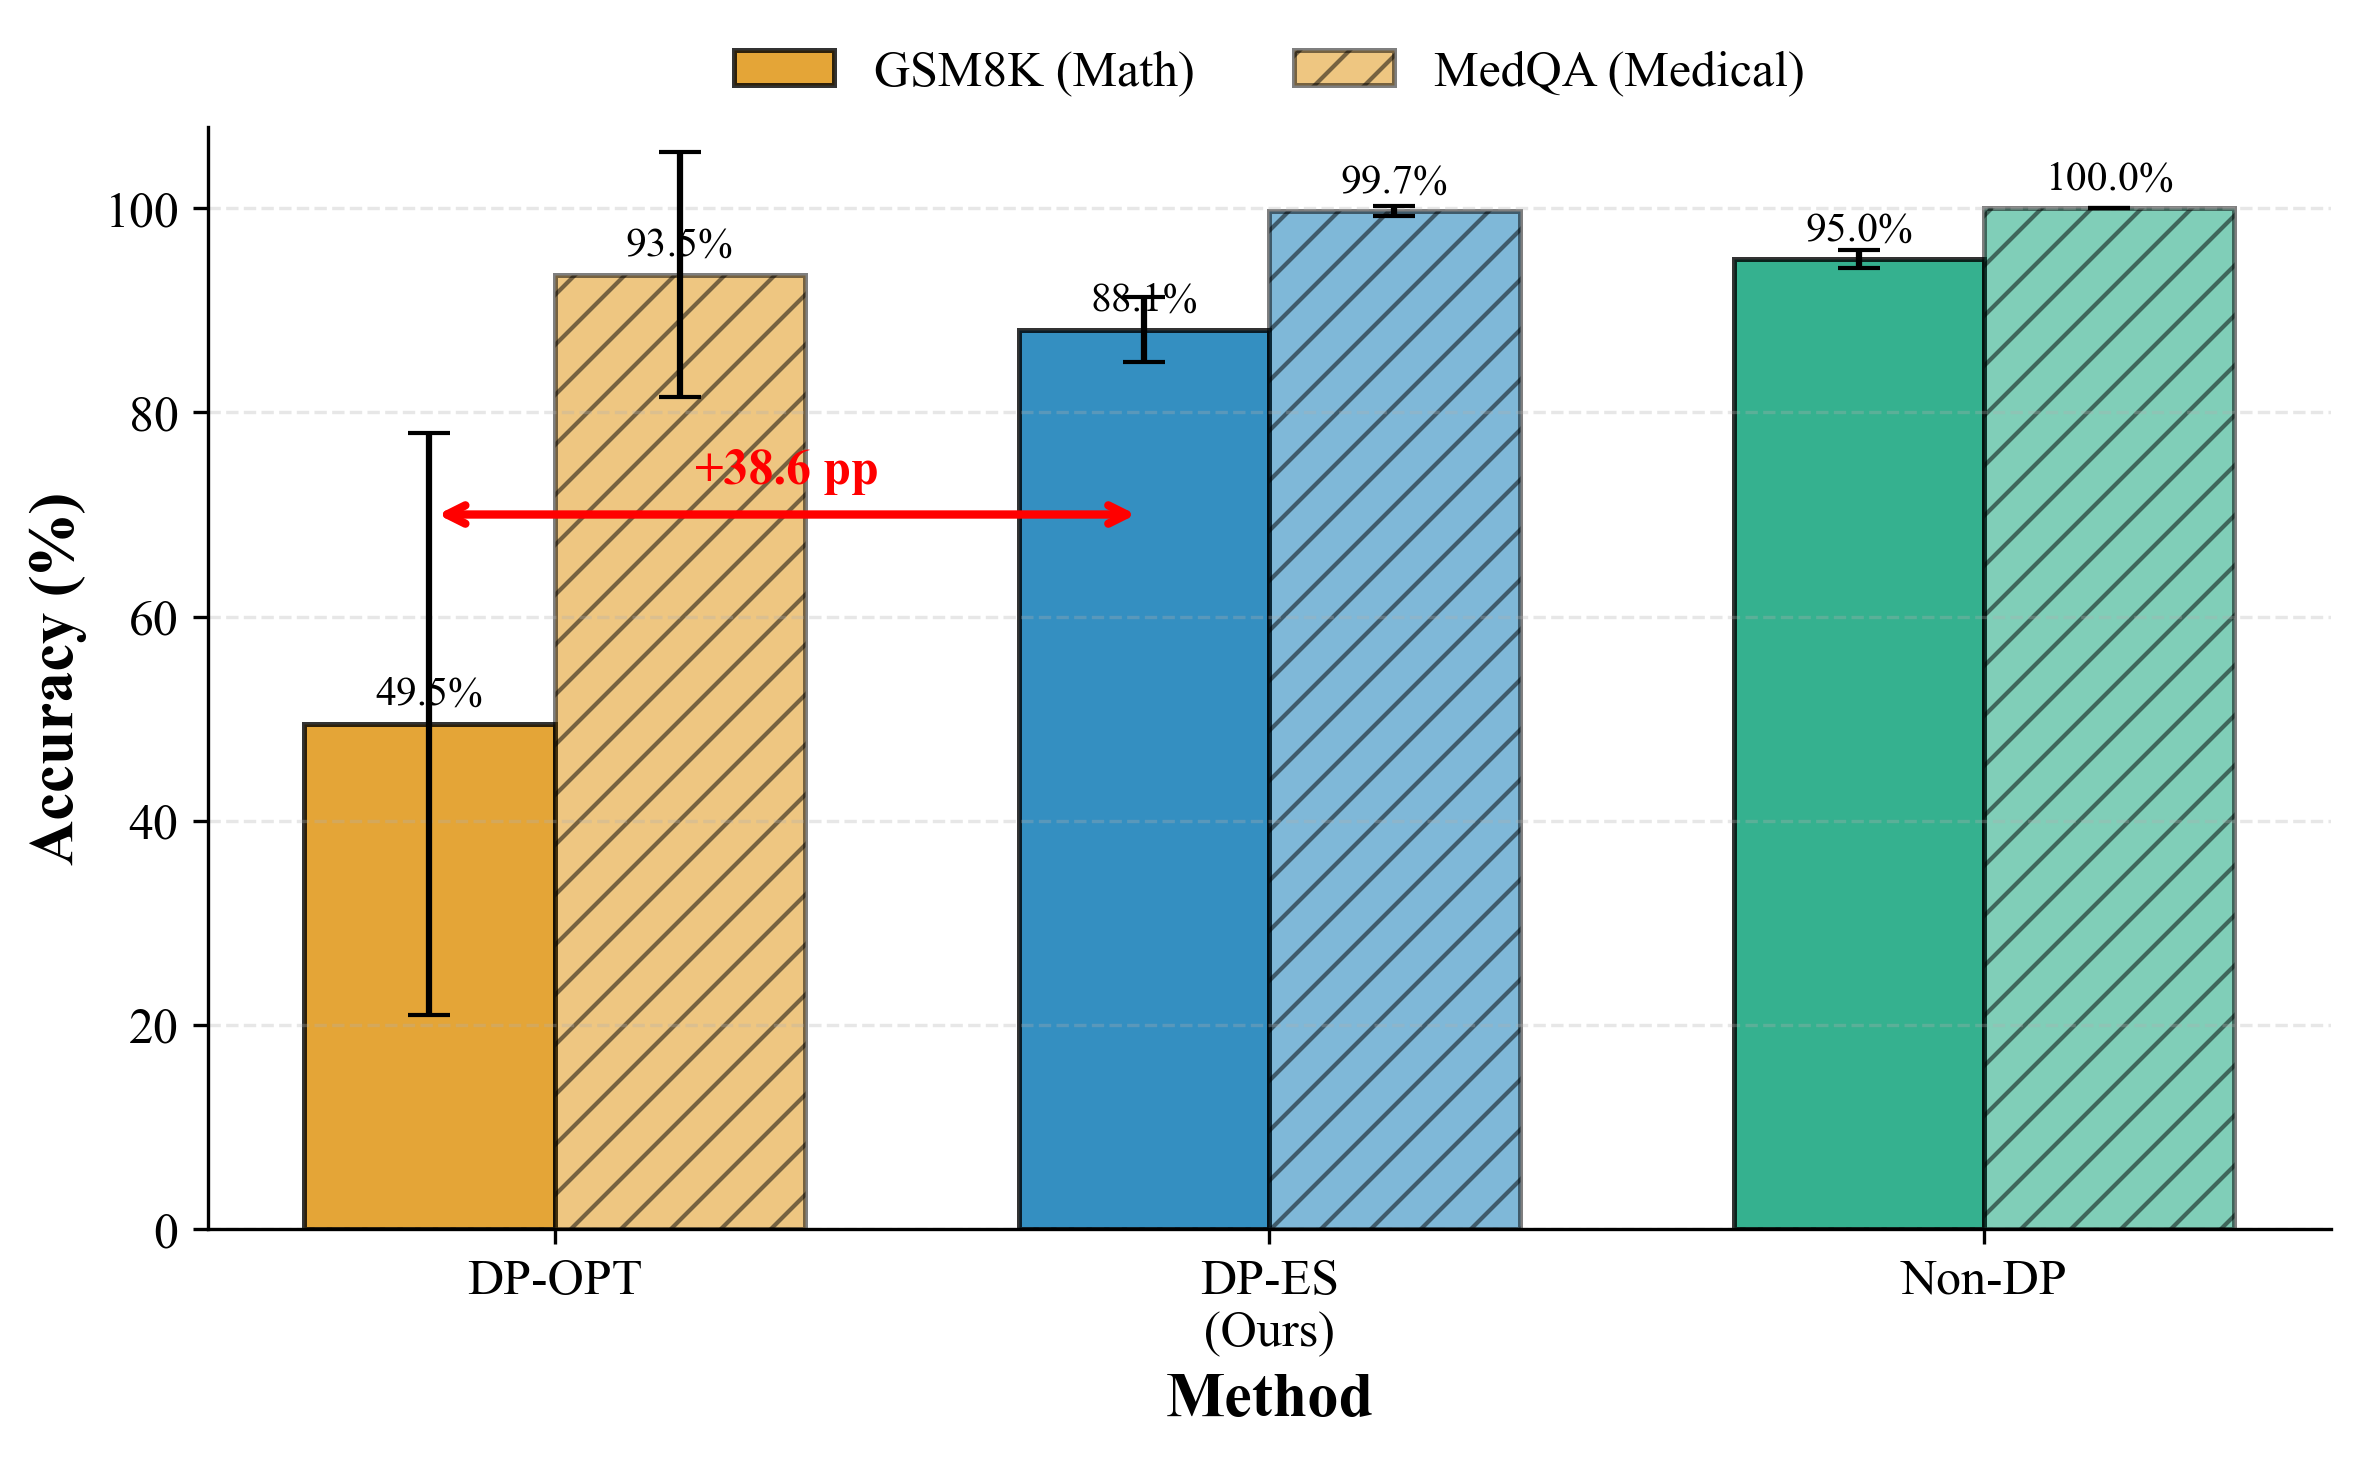
\includegraphics[width=\textwidth,height=0.55\textwidth]{figures/accuracy_comparison.png}
\end{subfigure}
\hfill
\begin{subfigure}[b]{0.48\textwidth}
    \centering
    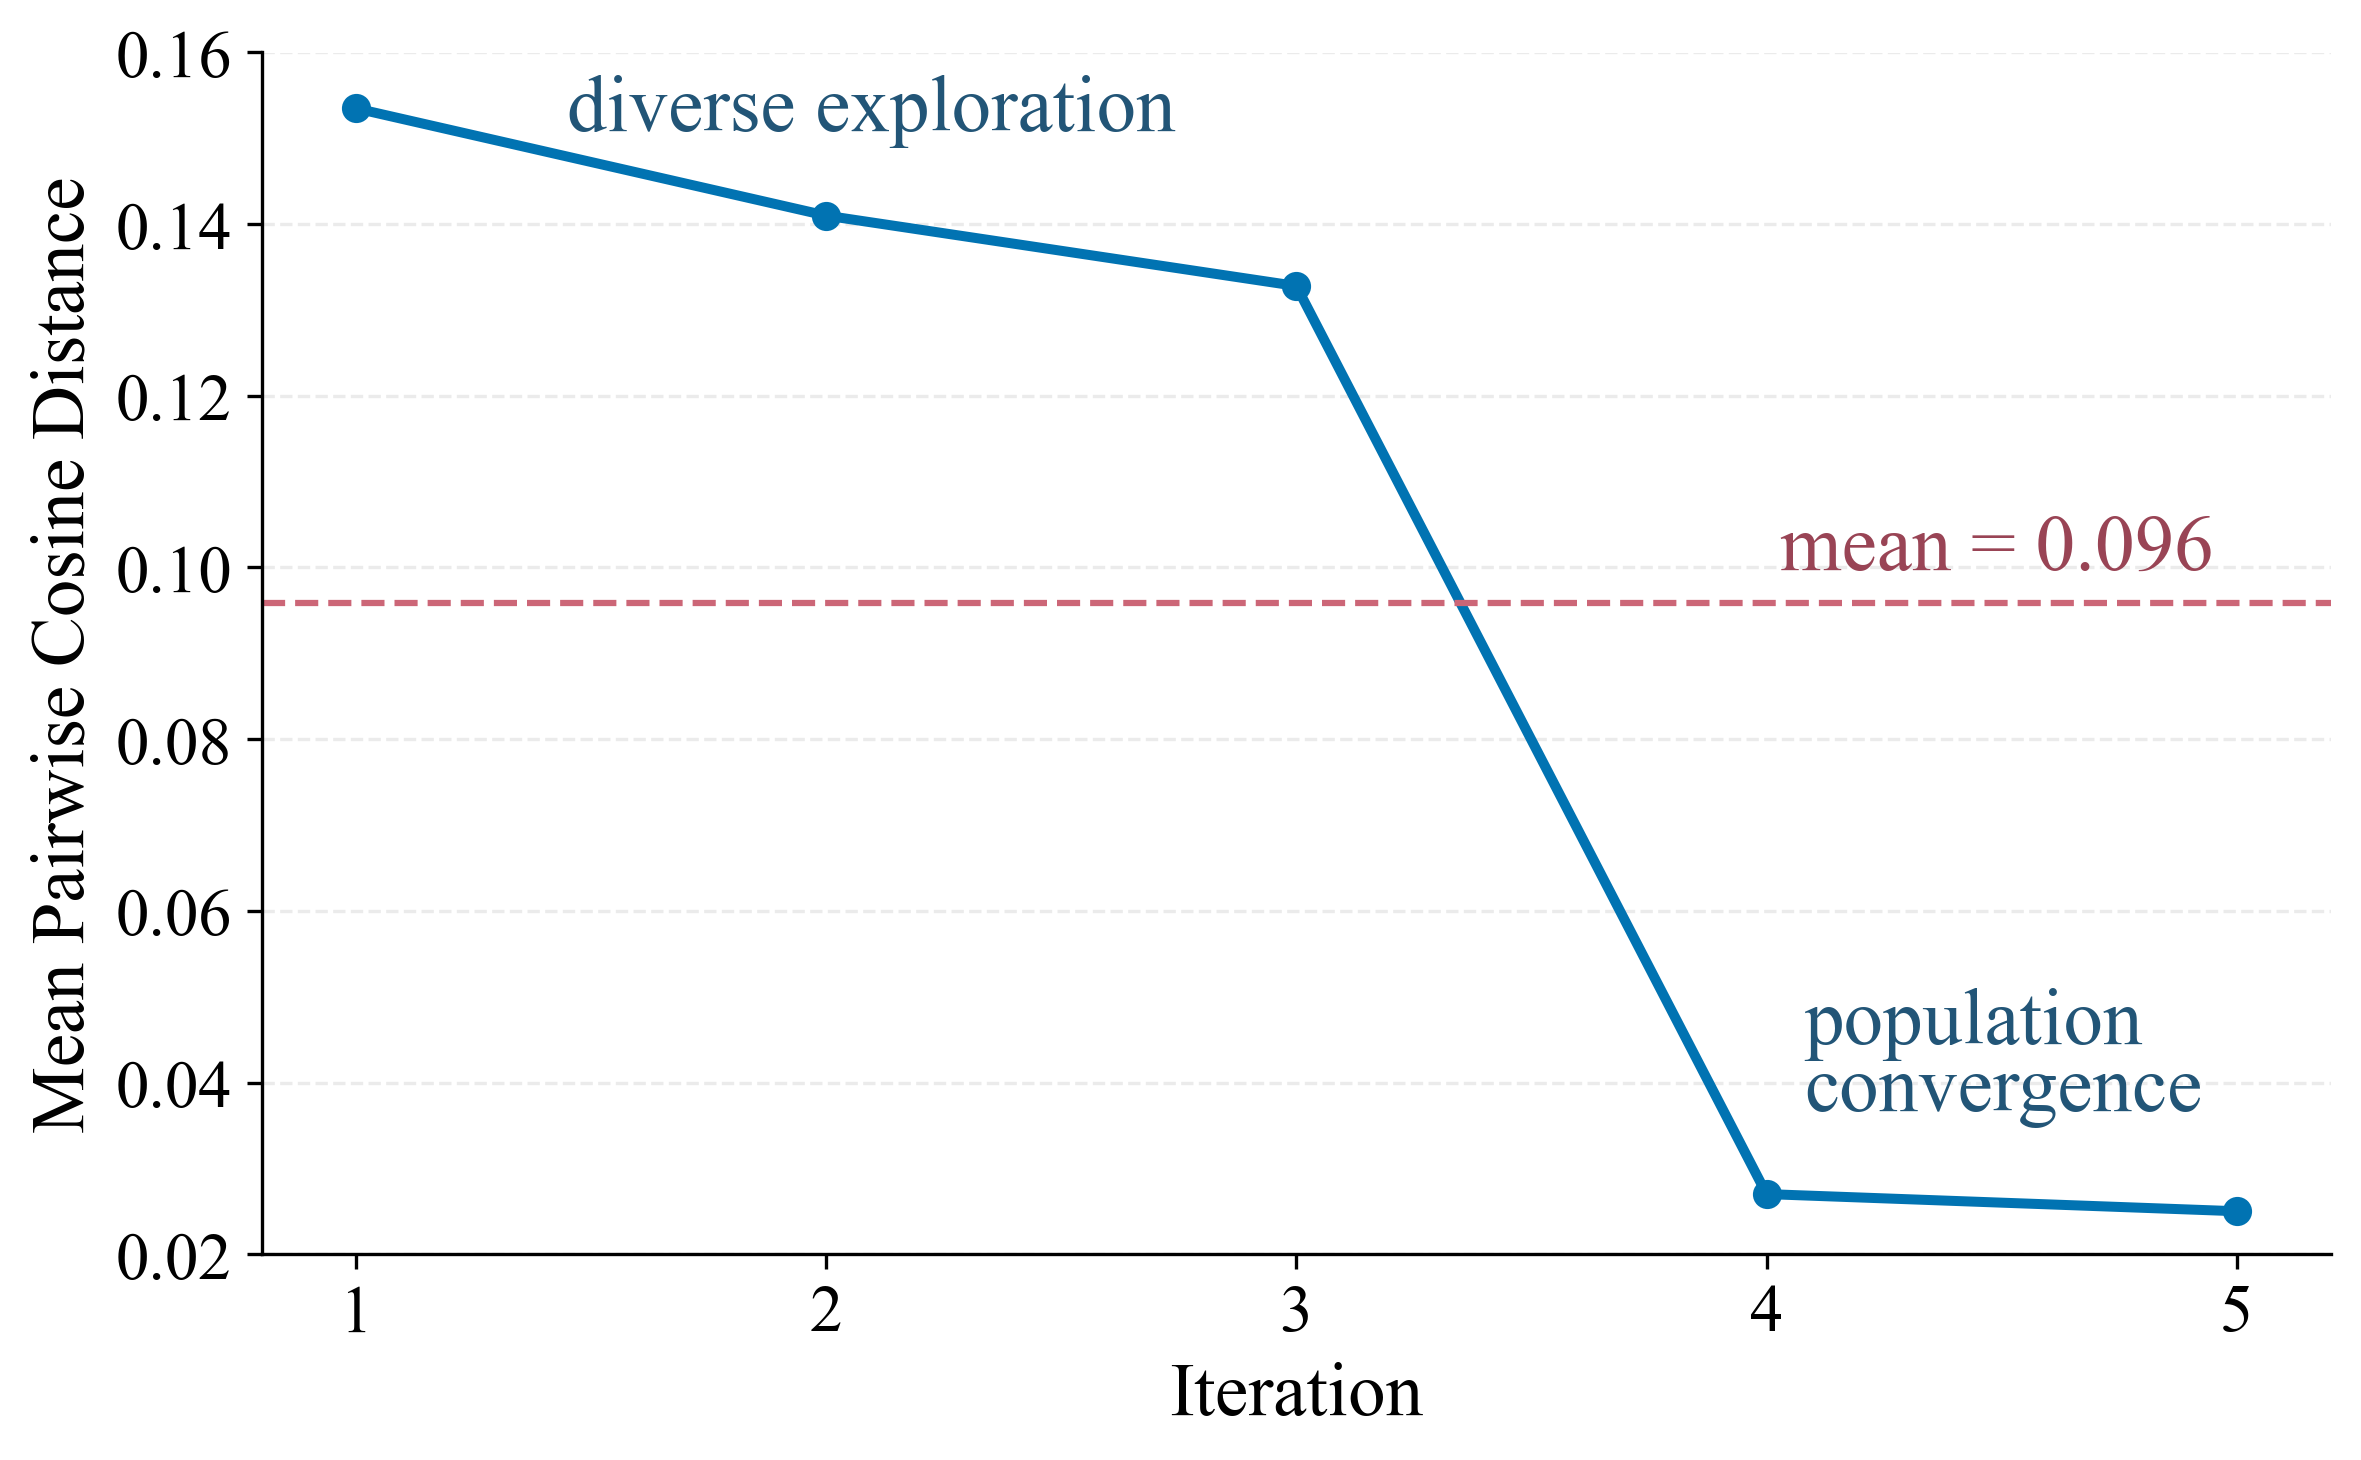
\includegraphics[width=\textwidth,height=0.55\textwidth]{figures/diversity_curve.png}
\end{subfigure}
\caption{\textbf{Performance and search dynamics.} \textbf{Left:} Accuracy on GSM8K and MedQA under the conservative $(\varepsilon{\leq}1,\delta{=}10^{-5})$ guarantee. \textbf{Right:} Mean pairwise prompt-embedding distance, showing early population diversity followed by convergence.}
\label{fig:performance_overview}
\end{figure*}
